\section{Anexo 3 - Wireshark logs}

\subsection{Experiência 1}

\begin{figure}[H]
\centering
  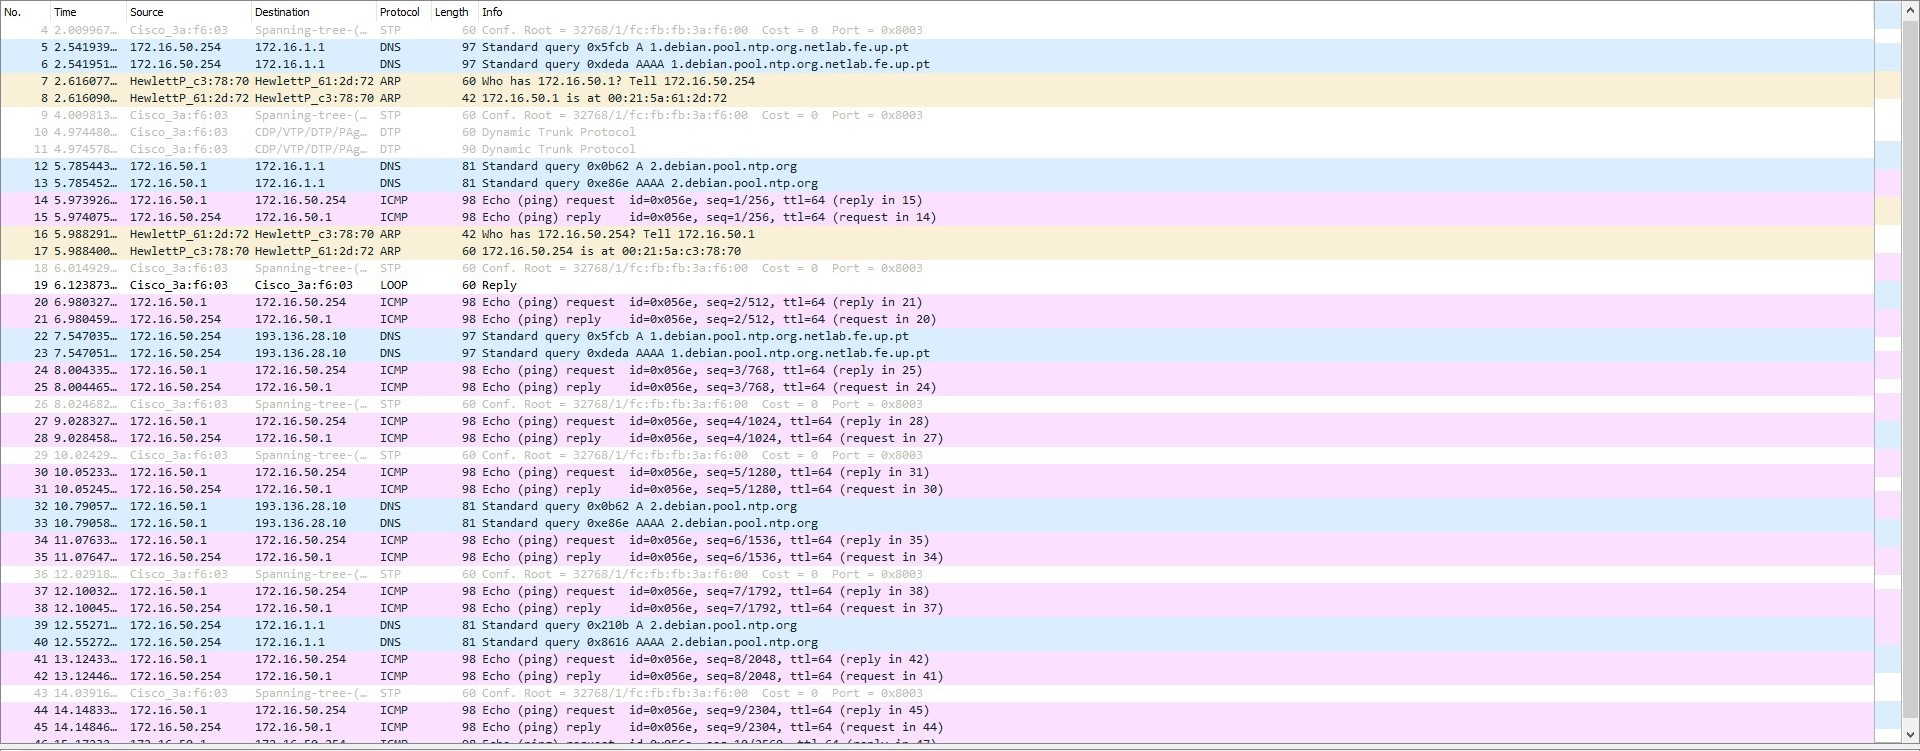
\includegraphics[width=\linewidth]{img/exp1.jpg}
  \caption{Experiência 1 - Resultado do ping de tux3 para tux4}
\end{figure}


\subsection{Experiência 2}

\begin{figure}[H]
\centering
  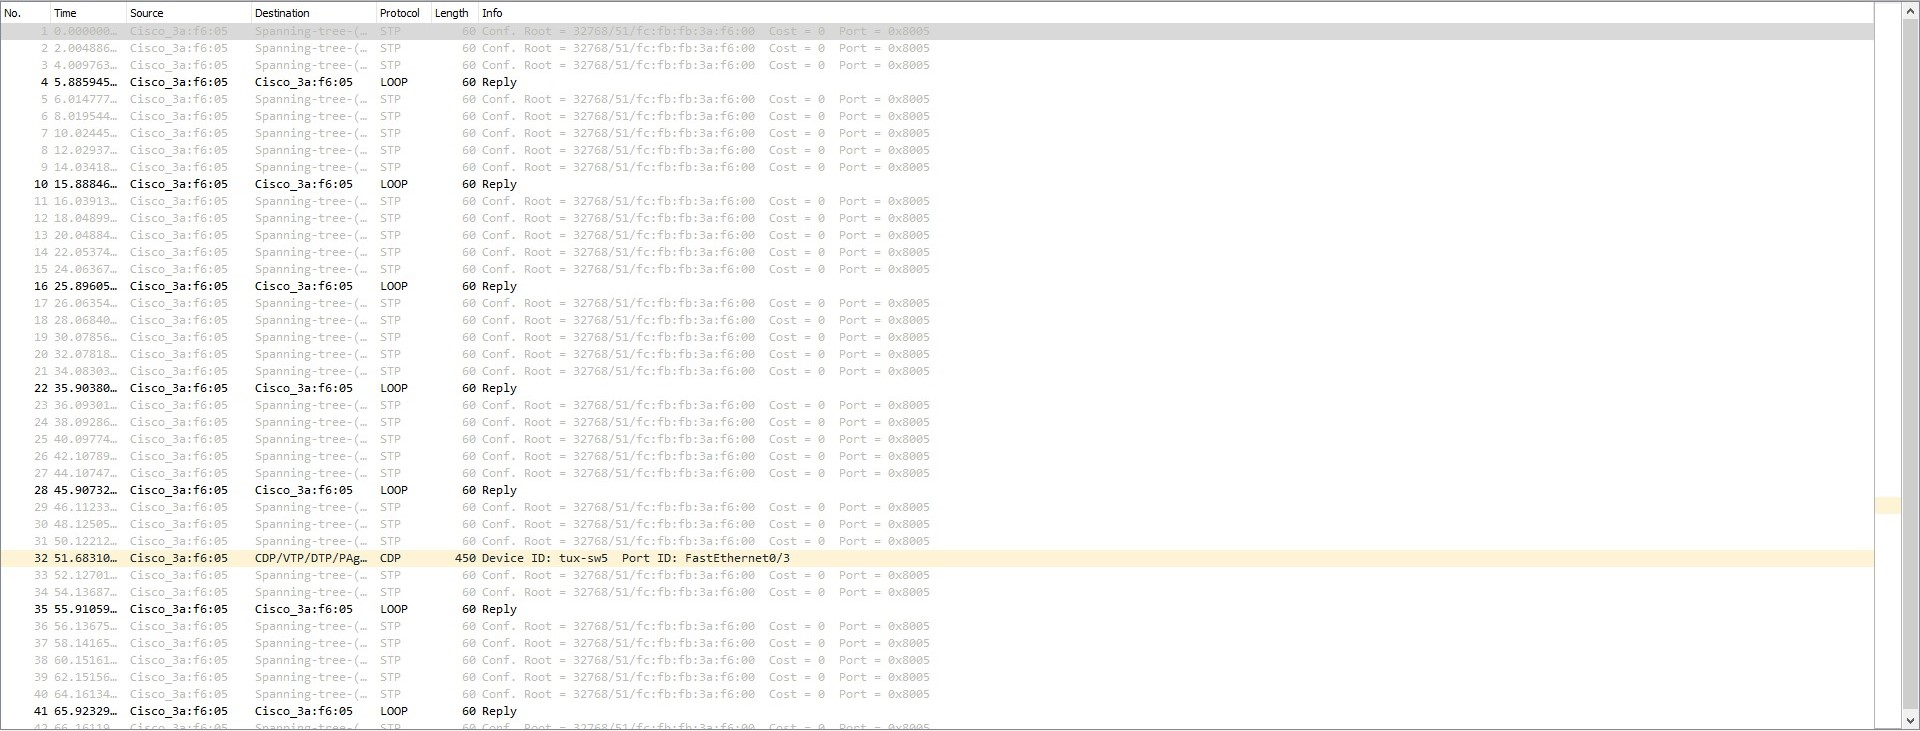
\includegraphics[width=\linewidth]{img/exp2-tsk8-tux2-full.jpg}
  \caption{Experiência 2 - Resultado do ping broadcast de tux3 em tux2}
\end{figure}

\begin{figure}[H]
\centering
  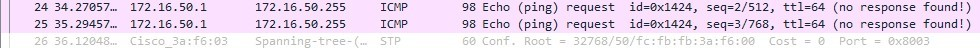
\includegraphics[width=\linewidth]{img/exp2-tsk8-tux3.jpg}
  \caption{Experiência 2 - tux3 ping broadcast tux3}
\end{figure}

\begin{figure}[H]
\centering
  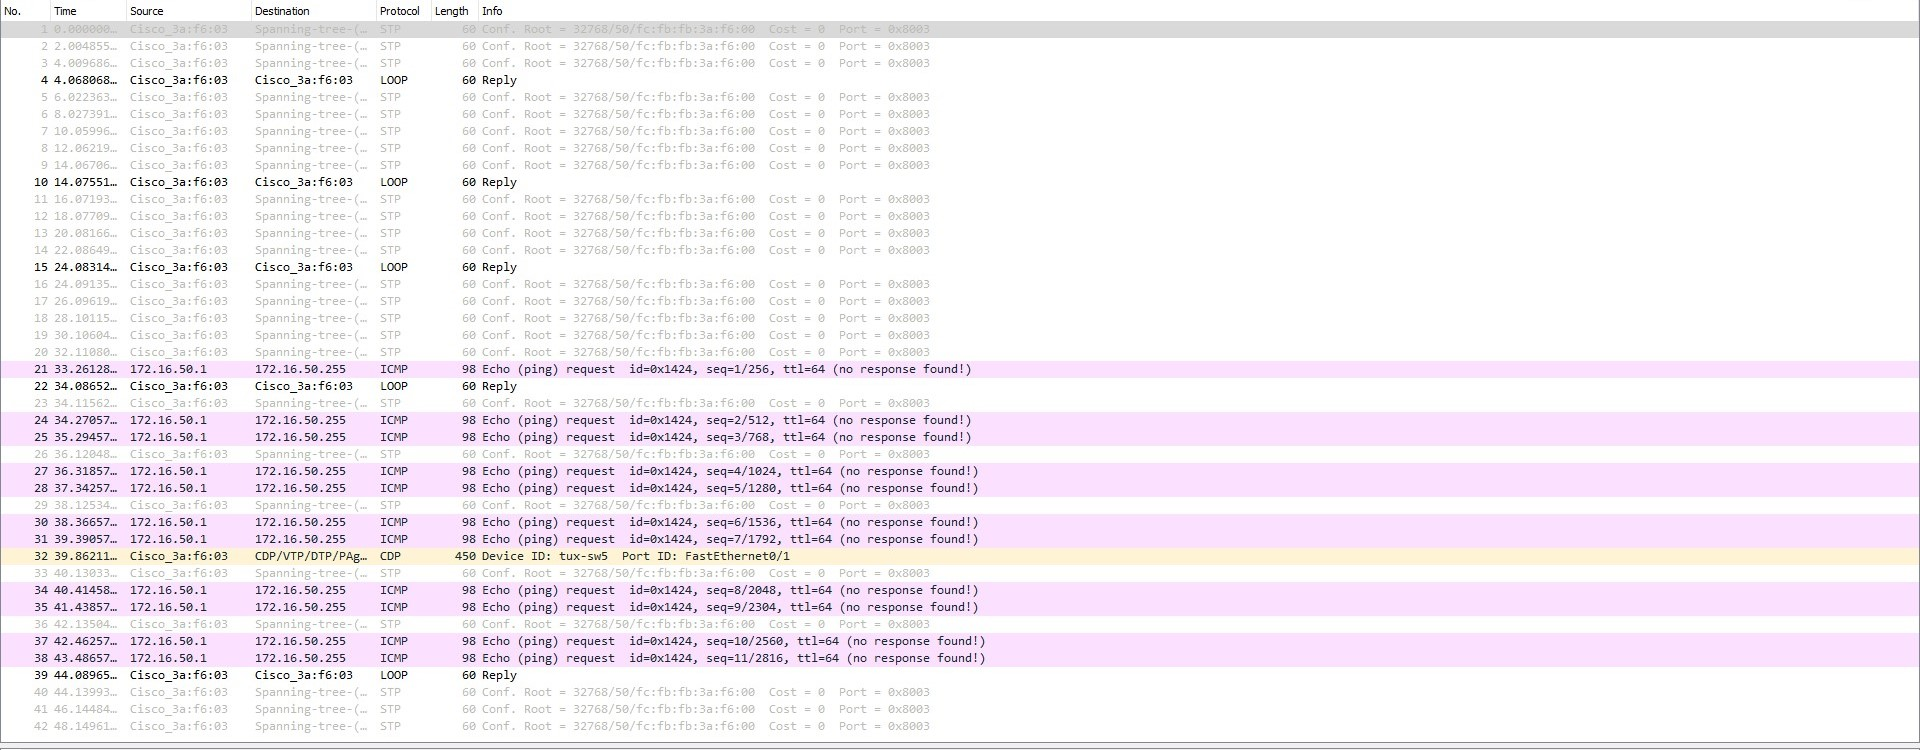
\includegraphics[width=\linewidth]{img/exp2-tsk8-tux3-full.jpg}
  \caption{Experiência 2 - Resultado do ping broadcast de tux3 em tux3}
\end{figure}

\begin{figure}[H]
\centering
  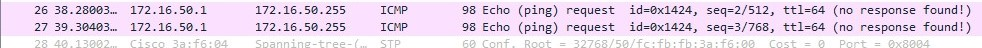
\includegraphics[width=\linewidth]{img/exp2-tsk8-tux4.jpg}
  \caption{Experiência 2 - tux3 ping broadcast tux4}
\end{figure}

\begin{figure}[H]
\centering
  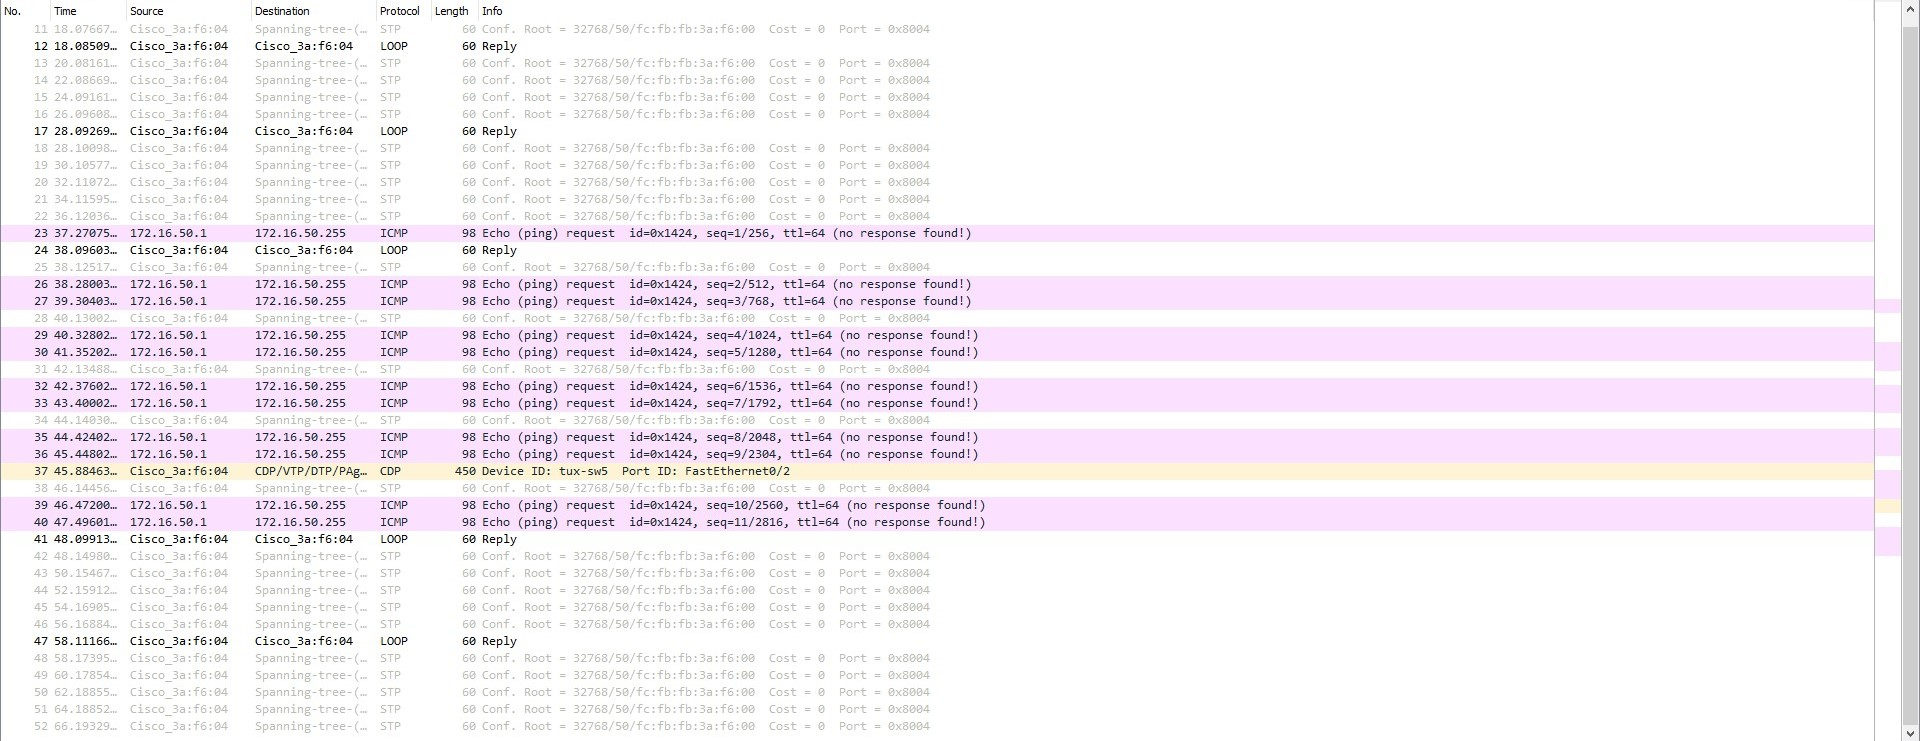
\includegraphics[width=\linewidth]{img/exp2-tsk8-tux4-full.jpg}
  \caption{Experiência 2 - Resultado do ping broadcast de tux3 em tux4}
\end{figure}

\begin{figure}[H]
\centering
  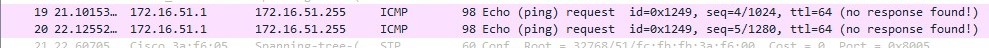
\includegraphics[width=\linewidth]{img/exp2-tsk10-tux2.jpg}
  \caption{Experiência 2 - tux2 ping broadcast}
\end{figure}

\begin{figure}[H]
\centering
  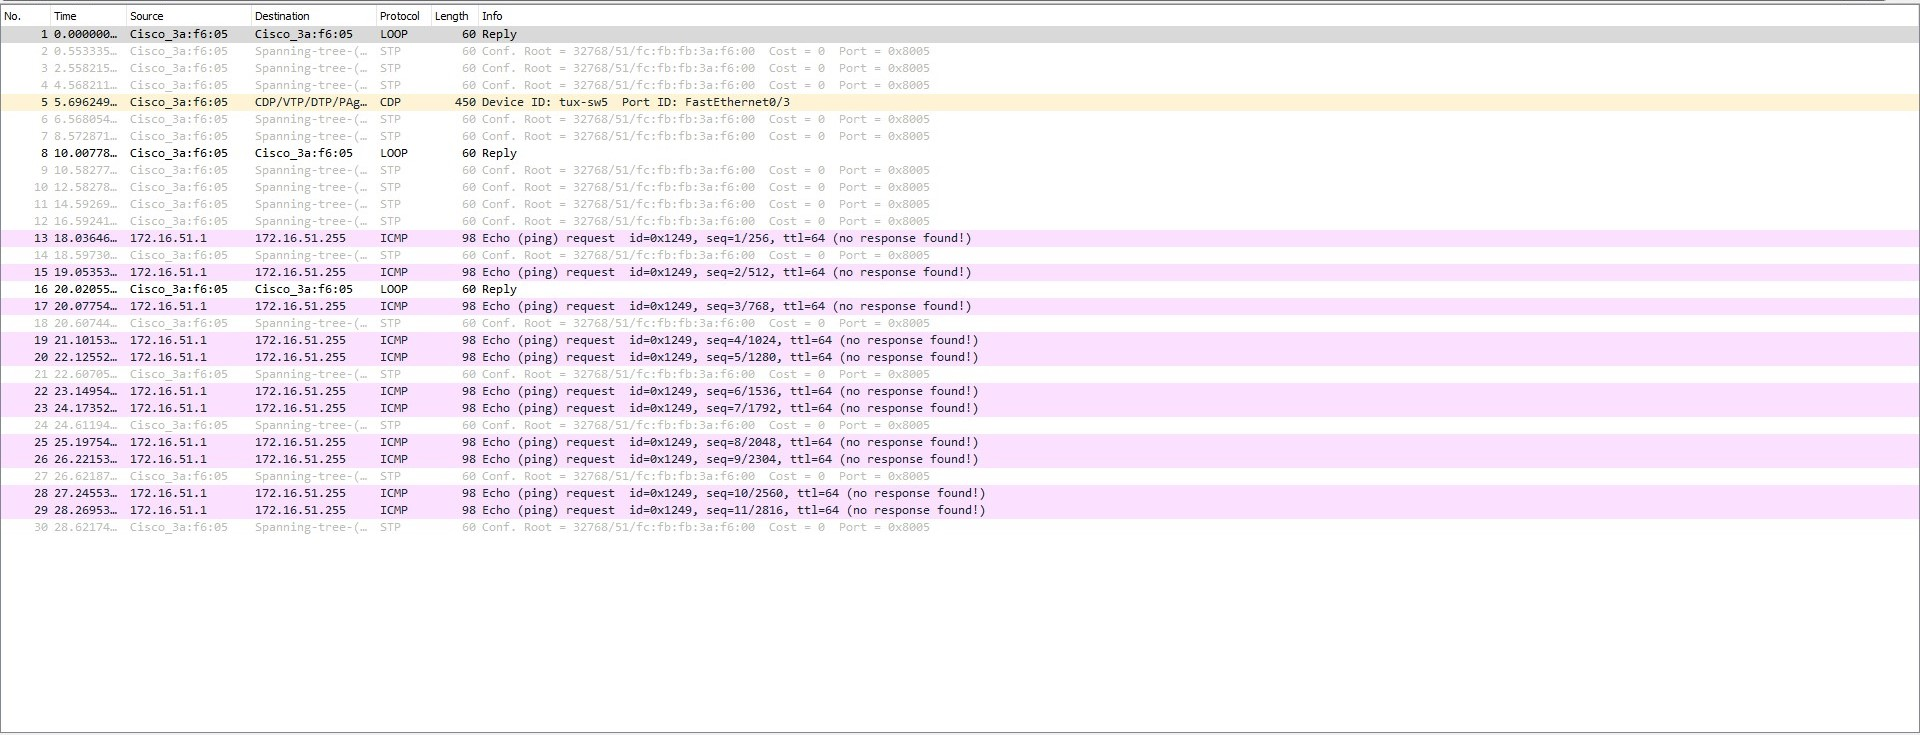
\includegraphics[width=\linewidth]{img/exp2-tsk10-tux2-full.jpg}
  \caption{Experiência 2 - Resultado do ping broadcast de tux2 em tux2}
\end{figure}

\begin{figure}[H]
\centering
  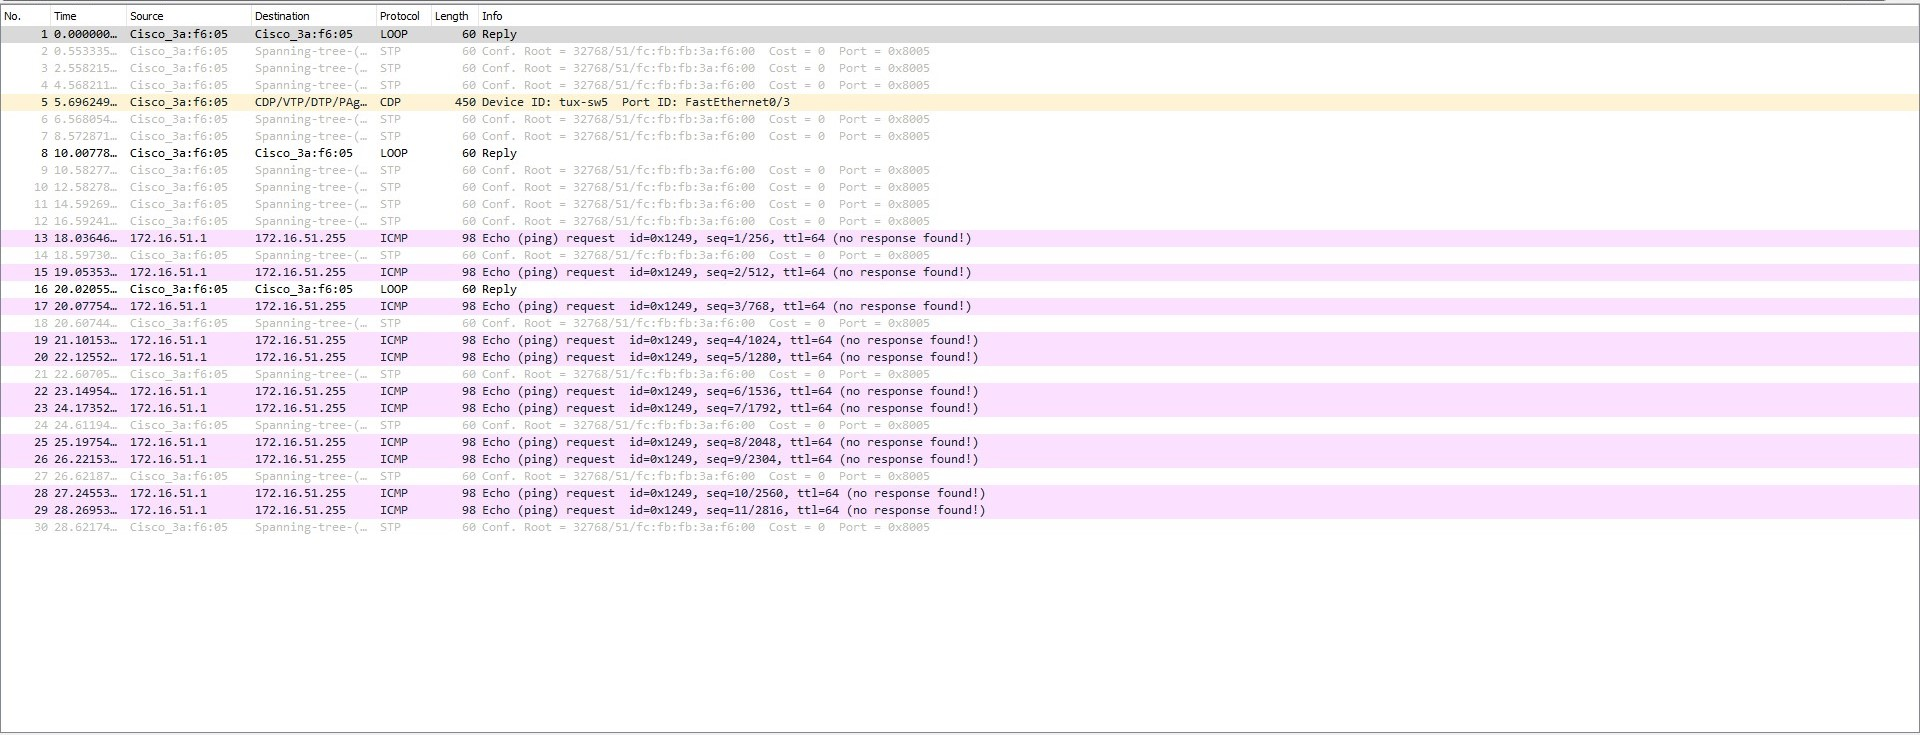
\includegraphics[width=\linewidth]{img/exp2-tsk10-tux2-full.jpg}
  \caption{Experiência 2 - Resultado do ping broadcast de tux2 em tux3}
\end{figure}

\begin{figure}[H]
\centering
  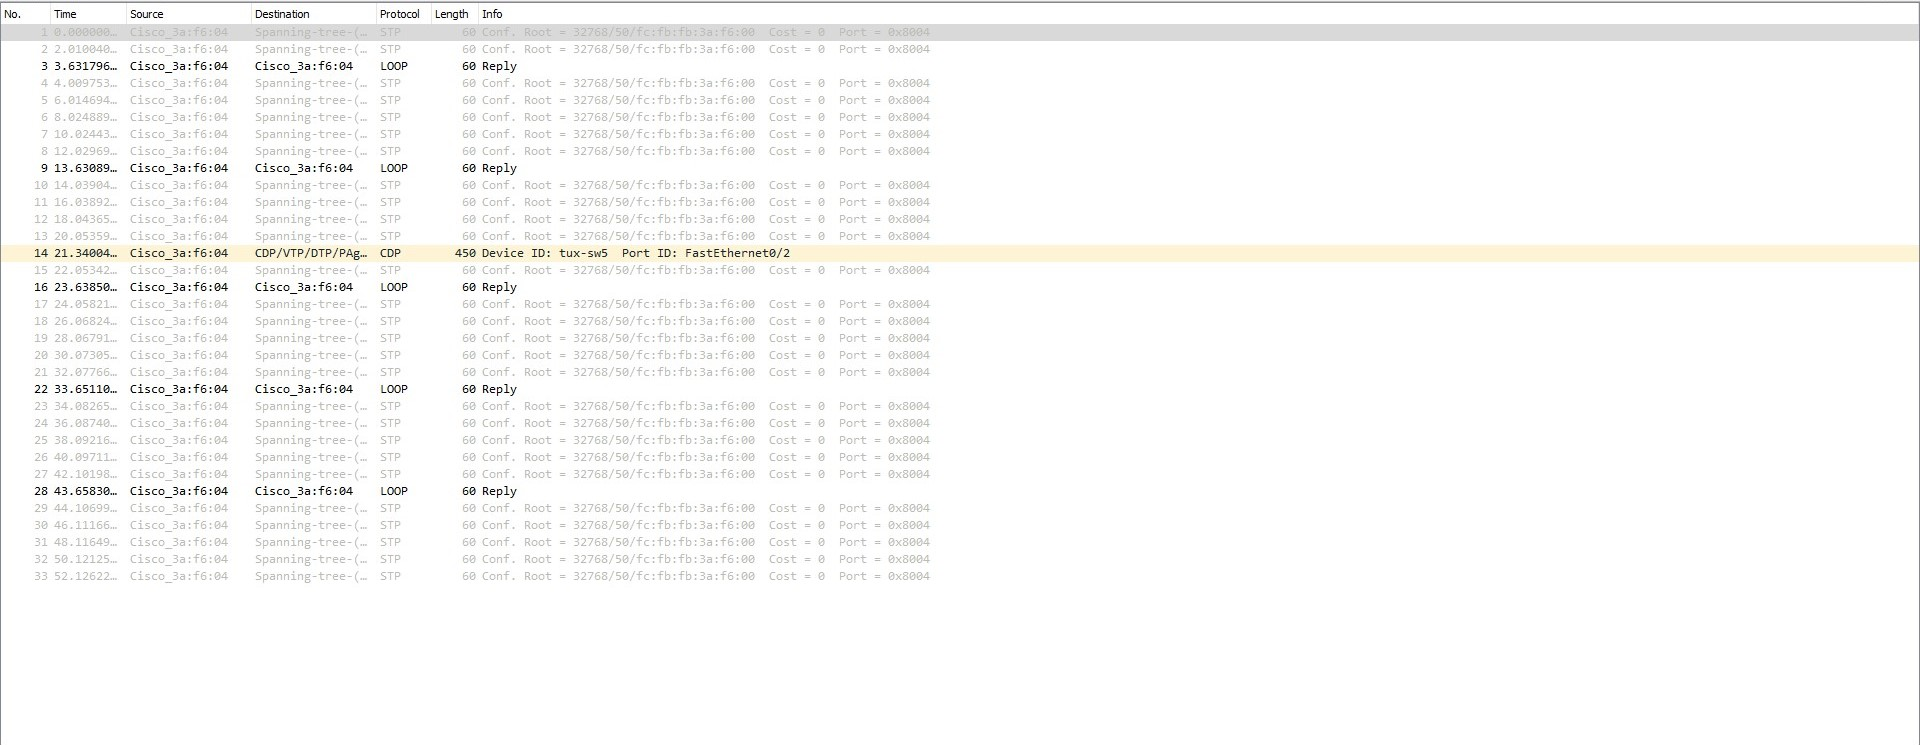
\includegraphics[width=\linewidth]{img/exp2-tsk10-tux4-full.jpg}
  \caption{Experiência 2 - Resultado do ping broadcast de tux2 em tux4}
\end{figure}


\subsection{Experiência 3}

\begin{figure}[H]
\centering
  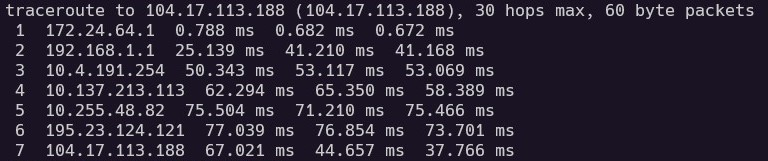
\includegraphics[width=\linewidth]{img/exp3-traceroute.jpg}
  \caption{Experiência 3 - Rota percorrida pelo pacote até atingir 104.17.113.188}
\end{figure}

\begin{figure}[H]
\centering
  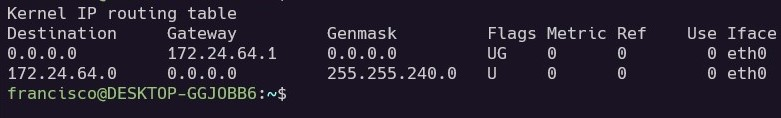
\includegraphics[width=\linewidth]{img/exp3-routes.jpg}
  \caption{Experiência 3 - Rotas presentes no computador}
\end{figure}

\begin{figure}[H]
\centering
  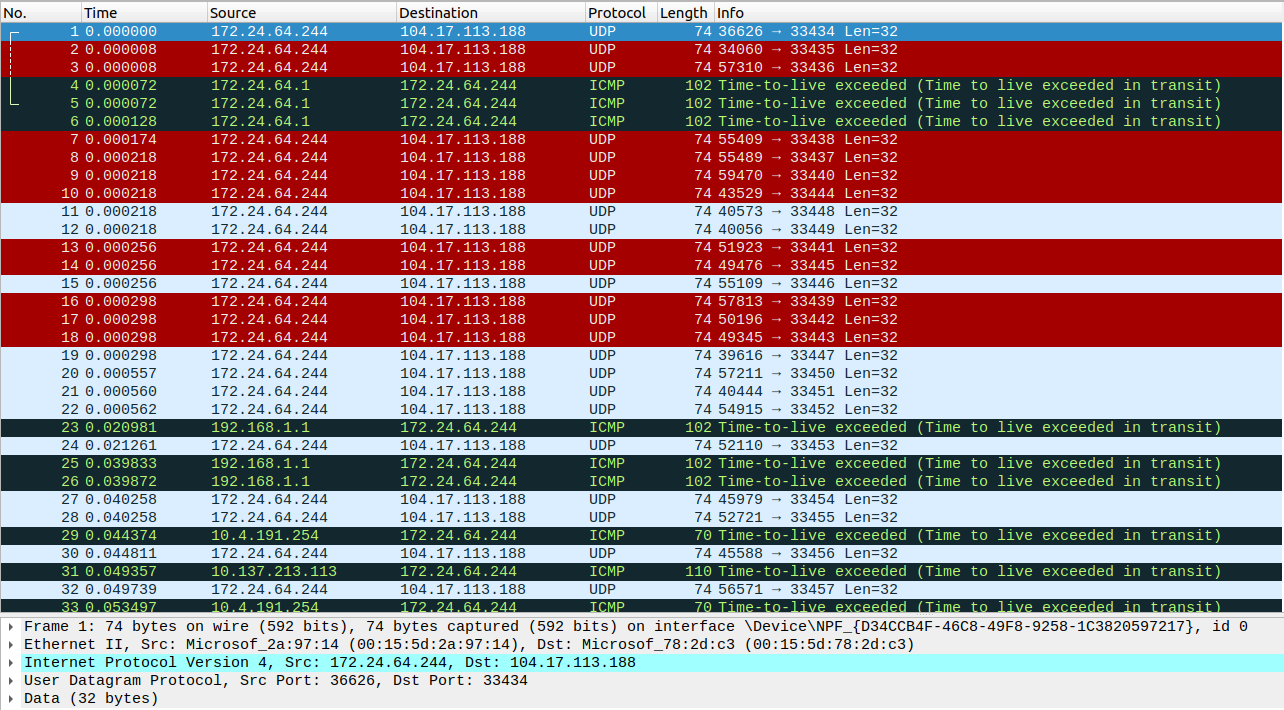
\includegraphics[width=\linewidth]{img/EXP3-traceroute.png}
  \caption{Experiência 3 - Resultado traceroute}
\end{figure}

\begin{figure}[H]
\centering
  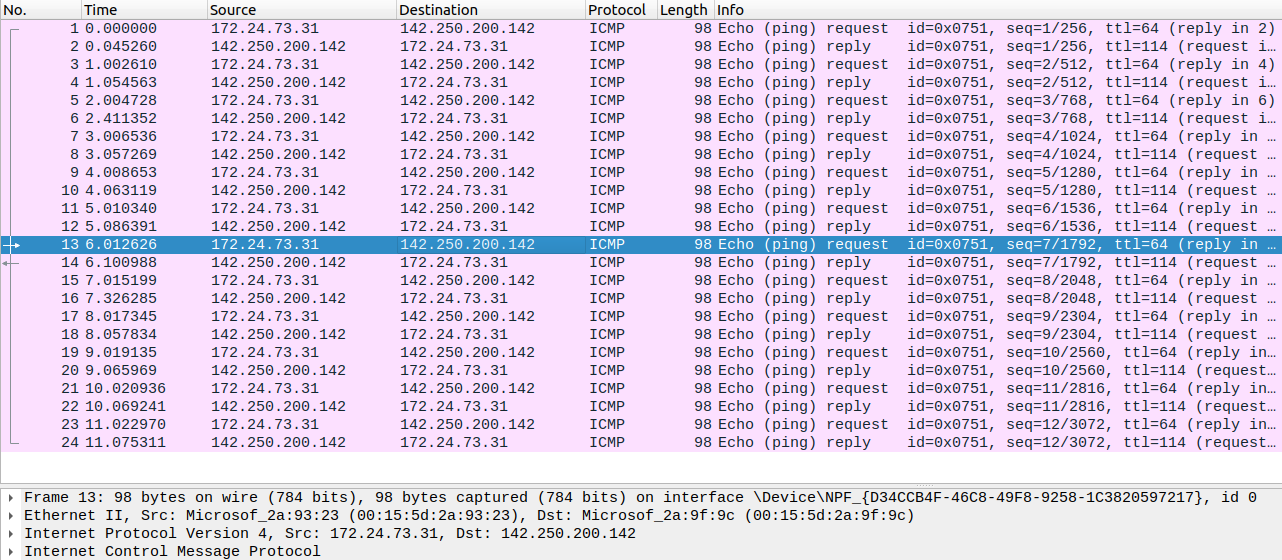
\includegraphics[width=\linewidth]{img/EXP3-youtubas.png}
  \caption{Experiência 3 - Resultado ping youtubas}
\end{figure}

\begin{figure}[H]
\centering
  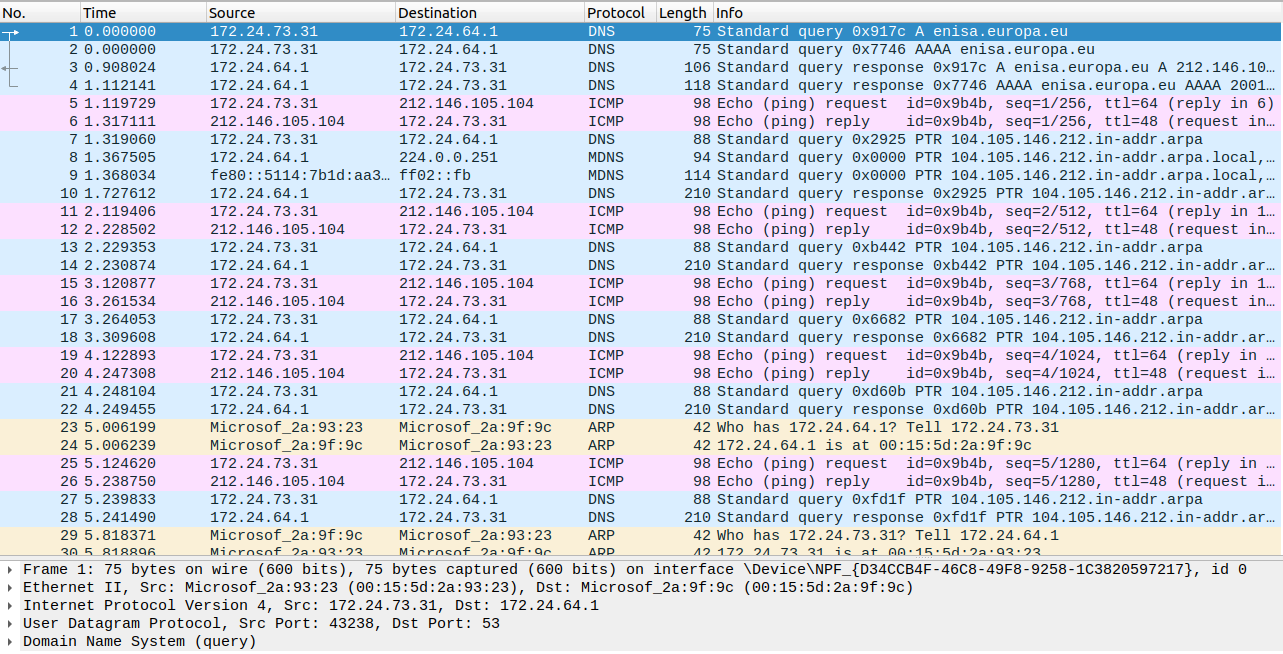
\includegraphics[width=\linewidth]{img/EXP3-enisa.png}
  \caption{Experiência 3 - Resultado ping enisa.europa.eu}
\end{figure}



\subsection{Experiência 4}

\begin{figure}[H]
\centering
  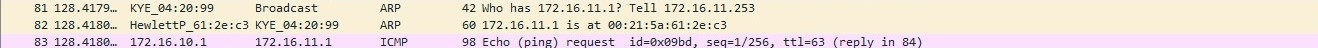
\includegraphics[width=\linewidth]{img/exp4-tux2-ask-tux4.jpg}
  \caption{Experiência 4 - tux4 pede MAC a tux2}
\end{figure}

\begin{figure}[H]
\centering
  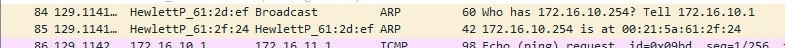
\includegraphics[width=\linewidth]{img/exp4-tux3-ask-tux4.jpg}
  \caption{Experiência 4 - tux3 pede MAC a tux4}
\end{figure}

\begin{figure}[H]
\centering
  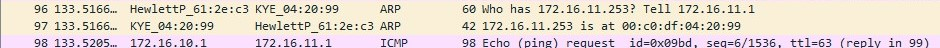
\includegraphics[width=\linewidth]{img/exp4-tux4-ask-tux2.jpg}
  \caption{Experiência 4 - tux2 pede MAC a tux4}
\end{figure}

\begin{figure}[H]
\centering
  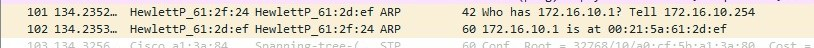
\includegraphics[width=\linewidth]{img/exp4-tux4-ask-tux3.jpg}
  \caption{Experiência 4 - tux4 pede MAC a tux3}
\end{figure}

\begin{figure}[H]
\centering
  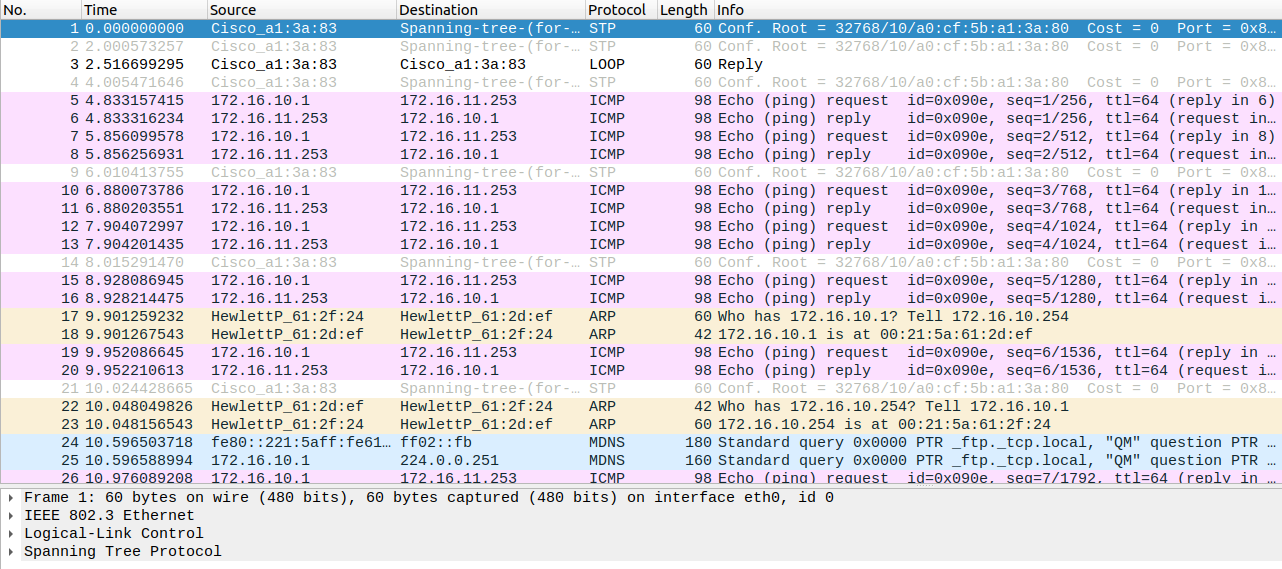
\includegraphics[width=\linewidth]{img/EXP4-3to4-253.png}
  \caption{Experiência 4 - Resultado de tux3 ping tux4 via 253}
\end{figure}

\begin{figure}[H]
\centering
  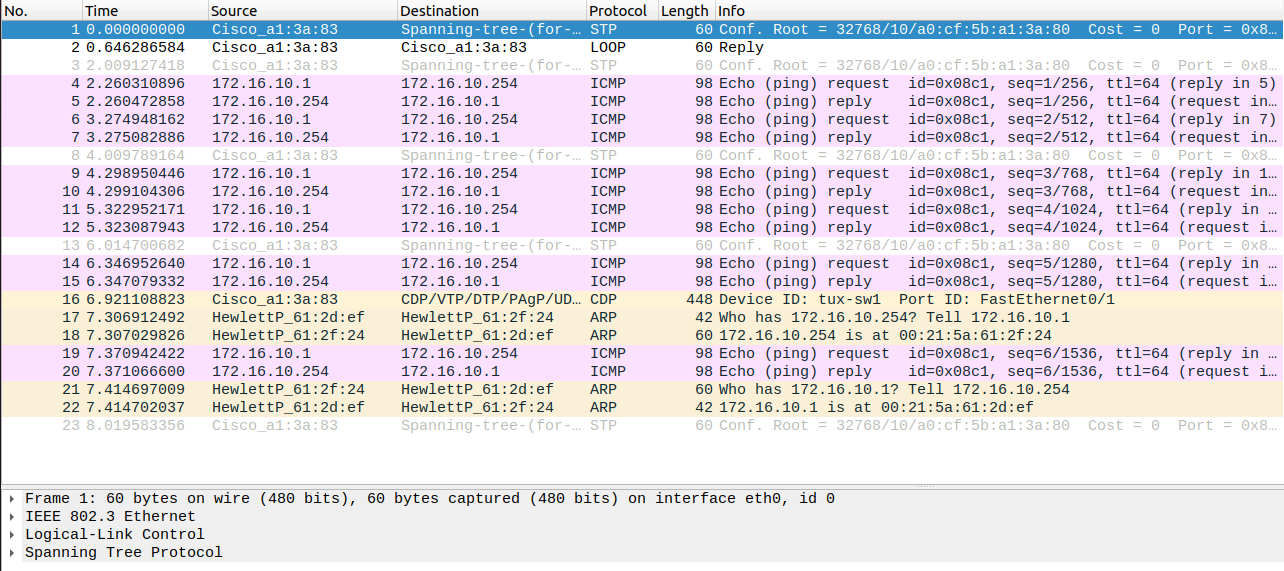
\includegraphics[width=\linewidth]{img/EXP4-3to4-254.png}
  \caption{Experiência 4 - Resulatdo de tux3 ping tux4 via 254}
\end{figure}

\begin{figure}[H]
\centering
  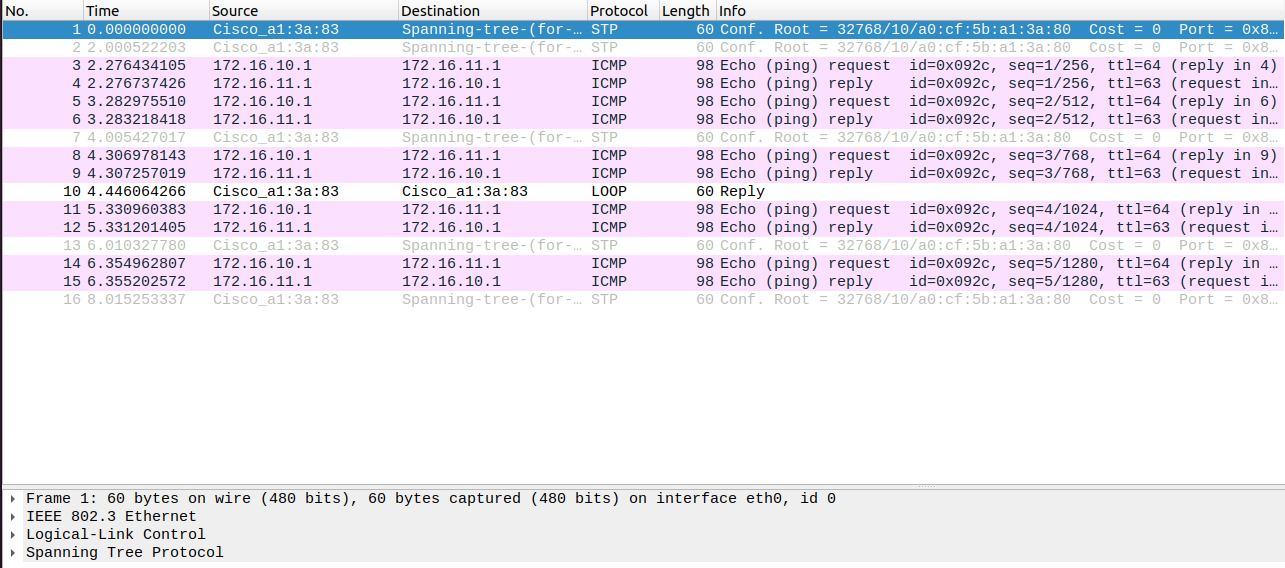
\includegraphics[width=\linewidth]{img/EXP4-3to2.png}
  \caption{Experiência 4 - Resultado de tux3 ping tux2}
\end{figure}

\begin{figure}[H]
\centering
  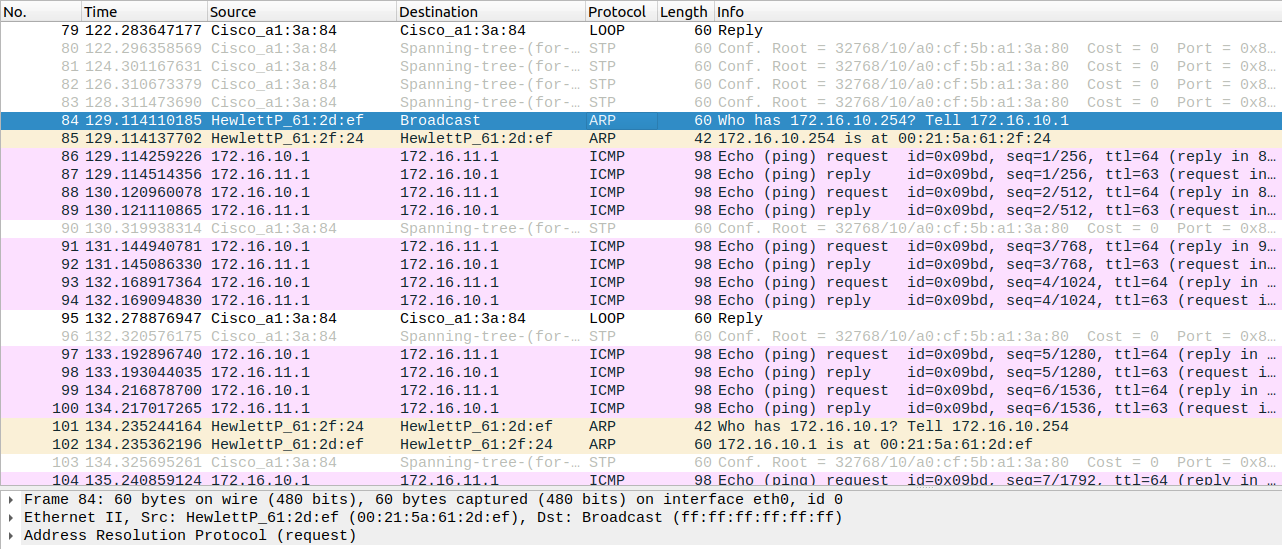
\includegraphics[width=\linewidth]{img/EXP4-task13-eth0.png}
  \caption{Experiência 4 - Resultado em tux4 eth0 de tux3 ping tux2}
\end{figure}

\begin{figure}[H]
\centering
  \includegraphics[width=\linewidth]{img/EXP4-task13-eth1.png}
  \caption{Experiência 4 - Resultado em tux4 eth1 de tux3 ping tux2}
\end{figure}


